\chapter{算法性能评估}
本章节主要讨论了关于之前三个算法性能的评估,包括GOP层面的优化,帧层面的优化,以及最后的GVBR算法。我们在所有的仿真实验中固定帧率为30帧每秒。

\section{最佳GOP}
\ref{sec:design_gop}章节的讨论表明减小关键帧间隔可以降低丢帧。在本节中,我们尝试去具体评估减少关键帧间隔所带来的性能优化。

\begin{figure}[H]% use float package if you want it here
  \centering
  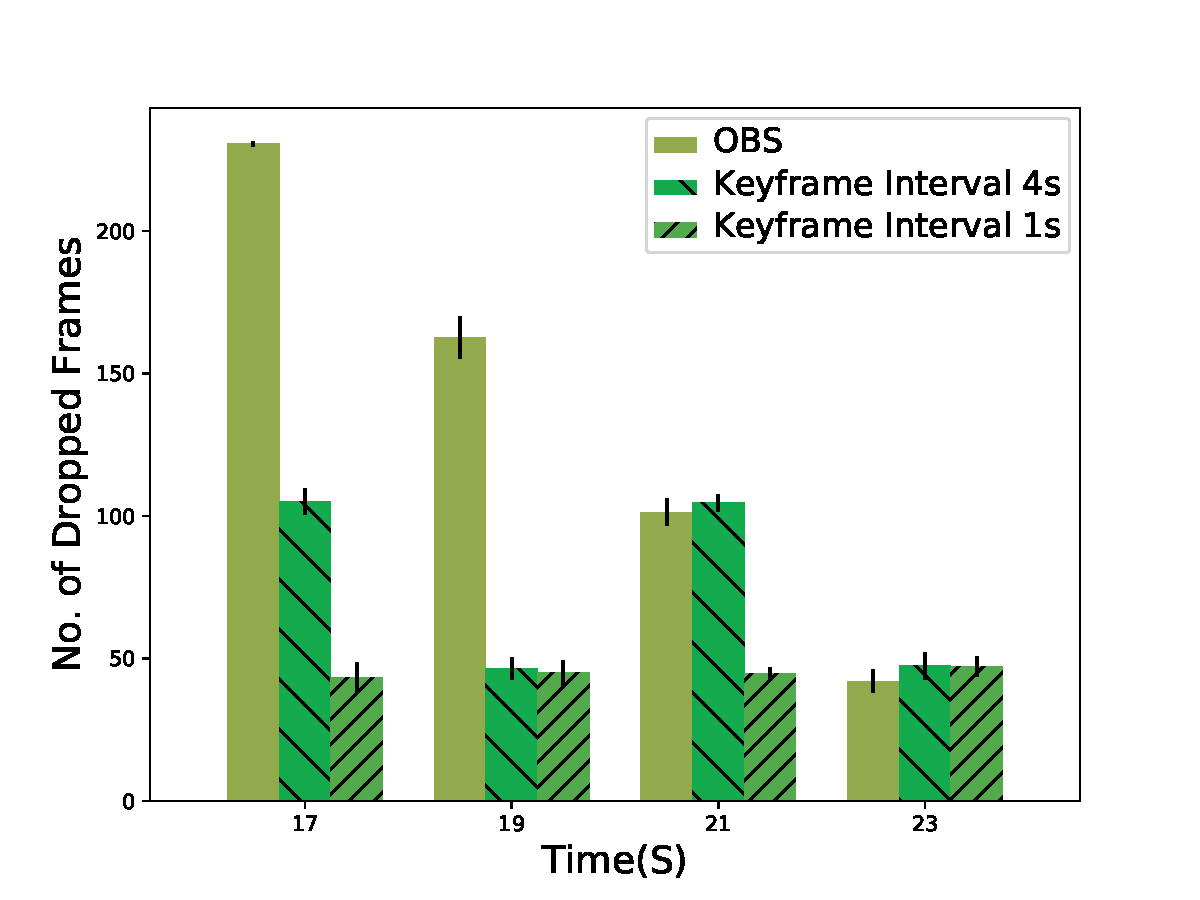
\includegraphics[width=\textwidth]{eval_IframeInterval_drop}
  \caption{不同关键帧间隔下的丢帧数}
  \label{fig:keyframe_drop}
\end{figure}

\textbf{改变关键帧间隔} OBS软件默认的关键帧间隔是8s,实验中我们把关键帧间隔分别改为4s和1s。每次实验,我们重复主播端推流的过程,使用同一个视频,在时间为0的时候开始上传视频。我们分别在时间为17s,19s,21s和23s的时候断开网络连接,断开时间为2s。丢帧的结果图展示在图~\ref{fig:keyframe_drop}。我们可以看到,对于关键帧相同的实验组来说,网络断开的时间处于一个GOP越早的时间,丢弃的帧数越多。因为GOP中较早的帧会有更多依赖于它的帧。对于默认为8s的关键帧间隔,当断开时间分别是17s,19s,21s和23s,丢帧数分别为238,164,105和48。对比在17s时断开的实验组,我们发现较小的关键帧间隔明显可以减少丢帧数,比如,当关键帧从8s变到4s再变到1s时,丢帧数从238减到102,最后减少到46。然后,23s的实验组,效果并不明显。这是因为23s在三组实验中均接近于GOP的尾部,只有1s的帧依赖于23s的帧。

实验结果表明,通过减少帧之间的依赖性,一个短暂的网络抖动只会丢弃抖动附近较短时间的帧,而不是产生放大效应,丢弃接下来好多秒的帧。

减少关键帧间隔是个很棘手的问题,因为减少可能会导致视频质量的降低。

\textbf{视频质量和关键帧} 前面提到过,关键帧的选择需要视频质量和丢帧之间的一个动态均衡。为了指导关键帧的选择,我们尝试去变化关键帧大小,将很多未压缩的视频流压缩成h264格式,测量每次实验的视频质量。实验使用x264编码器去编码,x264编码器使用差别编码模式。越大的关键帧间隔越有可能引起累计误差,GOP的推荐值是小于250帧。虽然有了一个最大值250帧的限制,决定具体的关键帧间隔值依然是很复杂。我们使用的视频数据集包含超清视频,高清视频,游戏和4k视频。关键帧间隔和归一化SSIM的关系展示在图~\ref{fig:ssim_gop}中。我们从众多结果中挑选出四个视频的编码结果,代表整体的实验结果。从图中可以看出,当关键帧间隔大于0.5s后,SSIM基本保持不变。结合上面的两部分测量,当关键帧大于0.5s,由于压缩量化导致的视频质量损失很微小;而小的关键帧间隔会减少丢帧。总结上面的实验,我们得出当关键帧的最佳选择是$[0.5,2]s$的范围。

\begin{figure}[htb]% use float package if you want it here
  \centering
  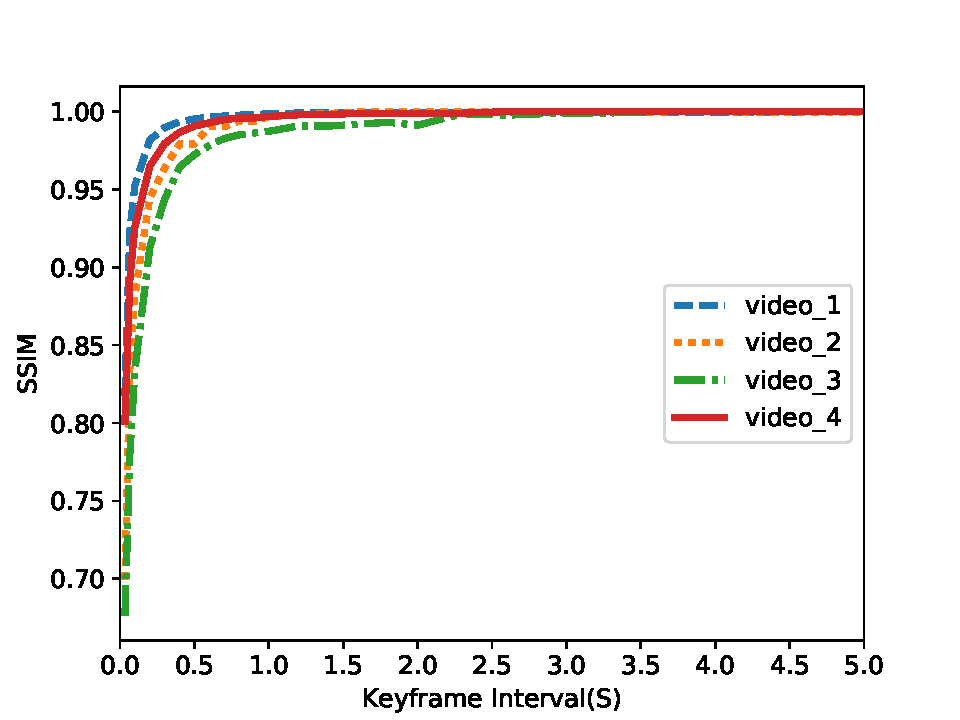
\includegraphics[width=\textwidth]{ssim_gop}
  \caption{不同关键帧间隔时视频编码后的SSIM}
  \label{fig:ssim_gop}
\end{figure}

\section{智能丢帧策略}
为了衡量算法的性能,我们对比了两个算法,离线最优算法Oracle和默认OBS算法。Oracle,通过暴力搜索达到离线最优,指数级的复杂度。我们从数据集中选择其中一段,时长30s。关键帧间隔选择上述给出的范围$[0.5,2]s$,我们选择为1s。为了研究算法优化丢帧的程度,我们将码率全程固定为2850kbps,使得选择的这段数据包含长时间的带宽抖动和带宽瞬时抖动。

\begin{figure}[htb]
  \centering%
  \begin{subfigure}{0.7\textwidth}
    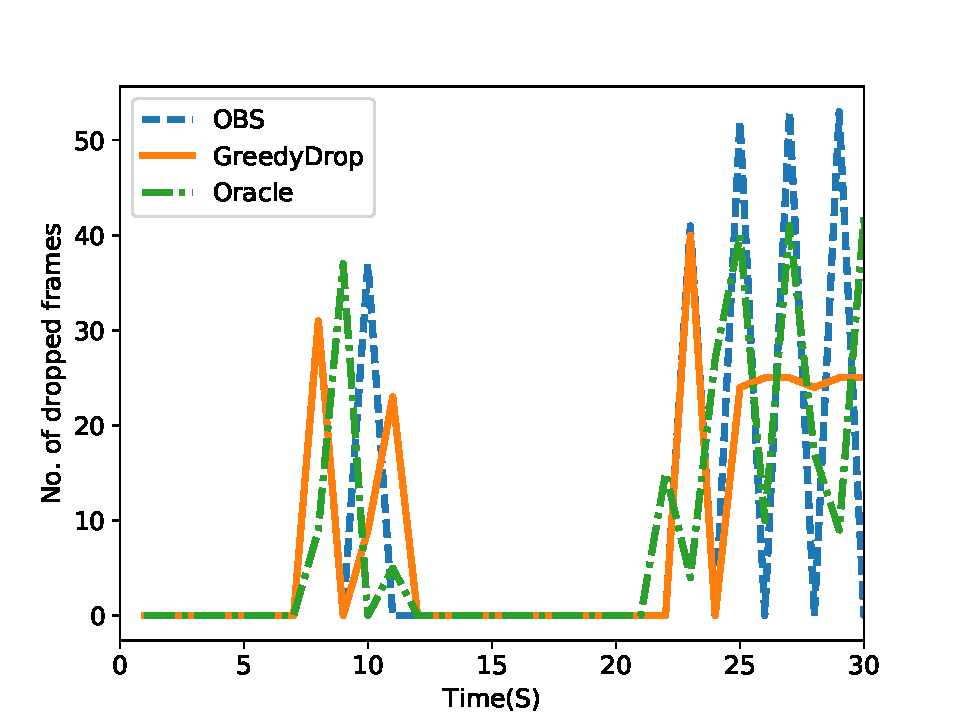
\includegraphics[width=\textwidth]{drop-buffer}
    \caption{实时丢帧数}
    \label{fig:drop-buffer}
  \end{subfigure}%
  \vfill
  \vspace{0.2in}
  \begin{subfigure}{0.7\textwidth}
    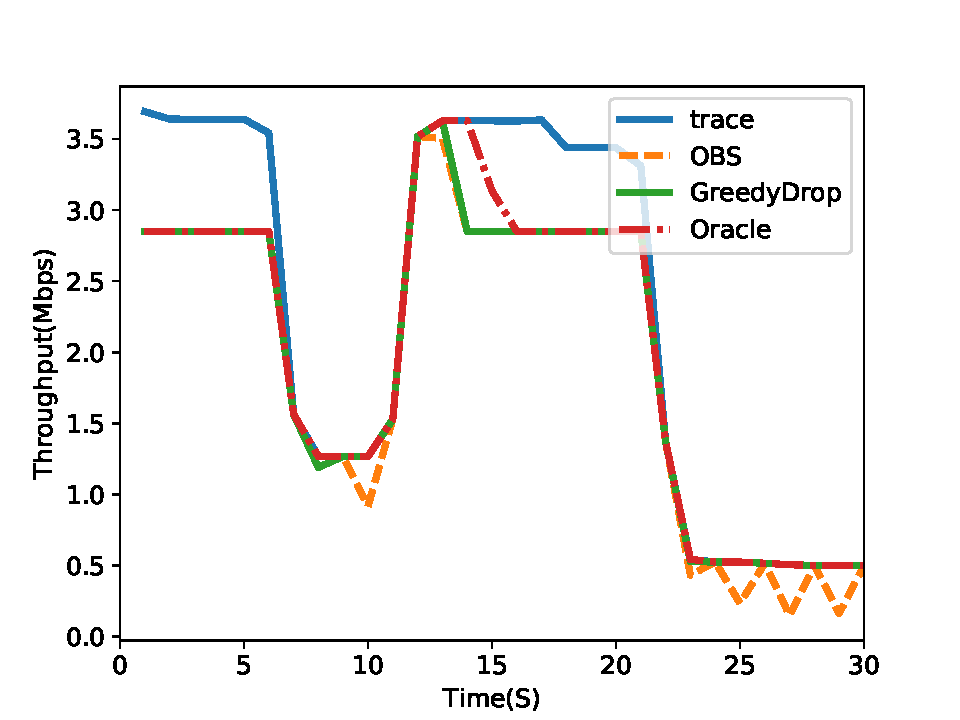
\includegraphics[width=\textwidth]{drop-bandwidth}
    \caption{实时的吞吐量}
    \label{fig:drop-bandwidth}
  \end{subfigure}
  \caption{不同丢帧策略性能比较}
  \label{fig:drop_comparison}
\end{figure}

丢帧的减少程度在表4中给出。上传失败时长定义为丢帧数对应的时长,即计算公式为上传失败时长=丢帧数/帧率。
OBS在三个算法中丢帧数最多,上传失败时长最长,GreedyDrop减少了15\%的上传失败,改善效果比较明显。而且GreedyDrop算法和离线最优Oracle算法之间的差距较小,小于5\%。丢帧和吞吐量的时序图展示在图~\ref{fig:drop_comparison}中。丢帧的主要时间段位于5-10s和20-30s。5-10s时三个算法的表现基本相同,但是Oracle会在视频队列中保存更多的有效帧,当网络恢复后,10-15s时Oracle会将队列中的视频帧发送出去,相比于其他两个算法,减少了一些丢帧。20-30s左右,OBS的丢帧数上下摆动,方差很大,而GreedyDrop算法基本每个时刻很稳定。因为GreedyDrop算法只丢掉视频队列中旧的GOP的帧。GreedyDrop算法中,对于每个GOP,开头的帧被发送出去,剩余的帧都被丢弃,规律性的行为使得丢帧和吞吐量都保持不动。Oracle也是每个时隙的丢帧数有一定的波动,但是变化比较小。同时考虑时间复杂度和算法性能,GreedyDrop是个不错的选择。


\section{自适应码率算法}
我们对比GVBR算法和三个在点播上表现很好的动态码率算法,我们用调和评估值来做带宽估计。
\begin{itemize}
  \item OBS-VBR:简单直接的码率自适应算法,每次都选择比估计带宽低的最高码率,除此之外,使用OBS默认的丢帧策略。
  \item MPC:用队列状态信息(帧数和帧的大小,以及帧的类型)和预测的带宽值去计算接下来几个时隙的最优码率选择,但只应用第一个时隙的码率选择。
  \item Robust-MPC:使用和MPC类似的方法,但是用过去几个时隙的最大预测误差去矫正带宽估计。
\end{itemize}
上述的算法使用GreedyDrop作为丢帧策略,除了OBS-VBR之外。Robust-MPC是视频点播领域最先进的码率自适应算法。默认预测控制理论,简称MPC,也可以直接应用到直播场景下。

\begin{figure}[htb]
  \centering%
  \begin{subfigure}{0.7\textwidth}
    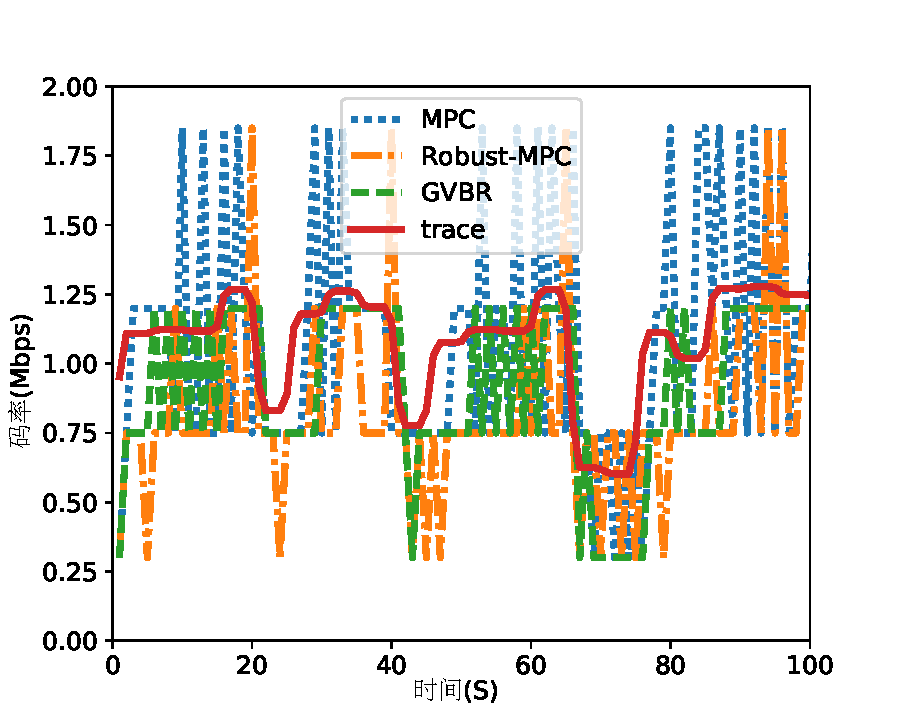
\includegraphics[width=\textwidth]{specific_fcc}
    \caption{FCC数据集的实时吞吐量}
    \label{fig:fcc}
  \end{subfigure}%
  \vfill
  \vspace{0.2in}
  \begin{subfigure}{0.7\textwidth}
    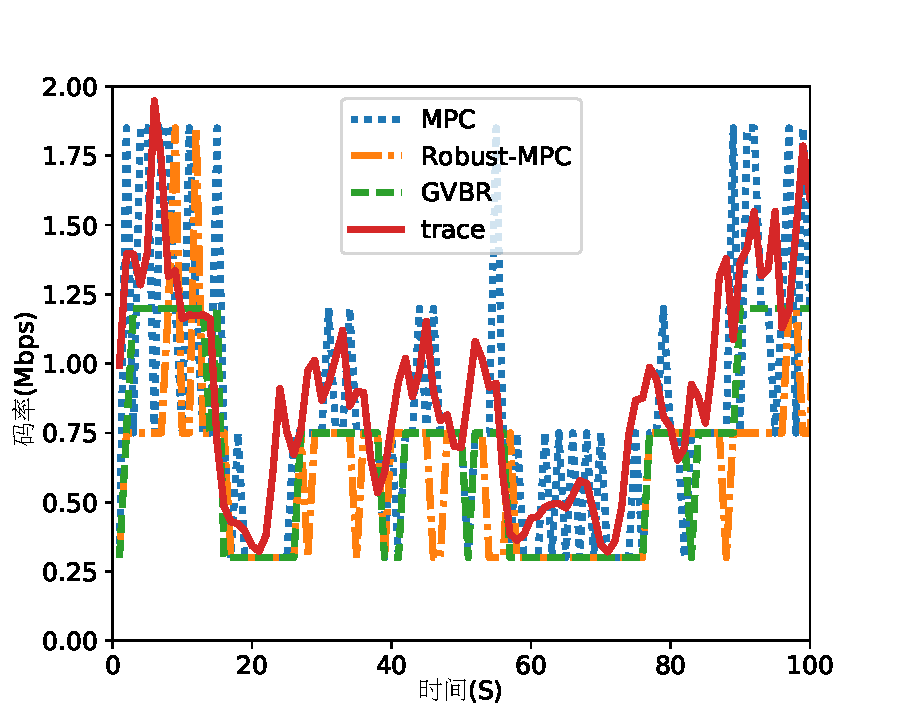
\includegraphics[width=\textwidth]{specific_hsdpa}
    \caption{HSDPA数据集的实时吞吐量}
    \label{fig:hsdpa}
  \end{subfigure}
  \caption{不同码率自适应算法吞吐量比较}
  \label{fig:specific}
\end{figure}

详细的对比算法结果展示在图~\ref{fig:specific}中。图~\ref{fig:fcc}和图~\ref{fig:hsdpa}分别对比了FCC数据集和HSDPA数据集下三种算法的性能。在这两幅图中,实线代表真实世界的带宽数据。相比于Robust-MPC,MPC缺少预测误差的矫正,容易更激进的选择更高的码率。除此之外,两个MPC算法的码率总是在真实带宽附近波动。两种情况下,MPC和Robust-MPC的码率切换都比GVBR更频繁。因为GVBR总是选择比带宽低的码率,当带宽波动较小时,GVBR很有发生变化。但是MPC总是选择一个使效益最高的码率,当带宽稍微增加一点,MPC会更加倾向于选择一个更高的码率,增大优化目标中的第一项,码率效益。

\begin{figure}[htb]% use float package if you want it here
  \centering
  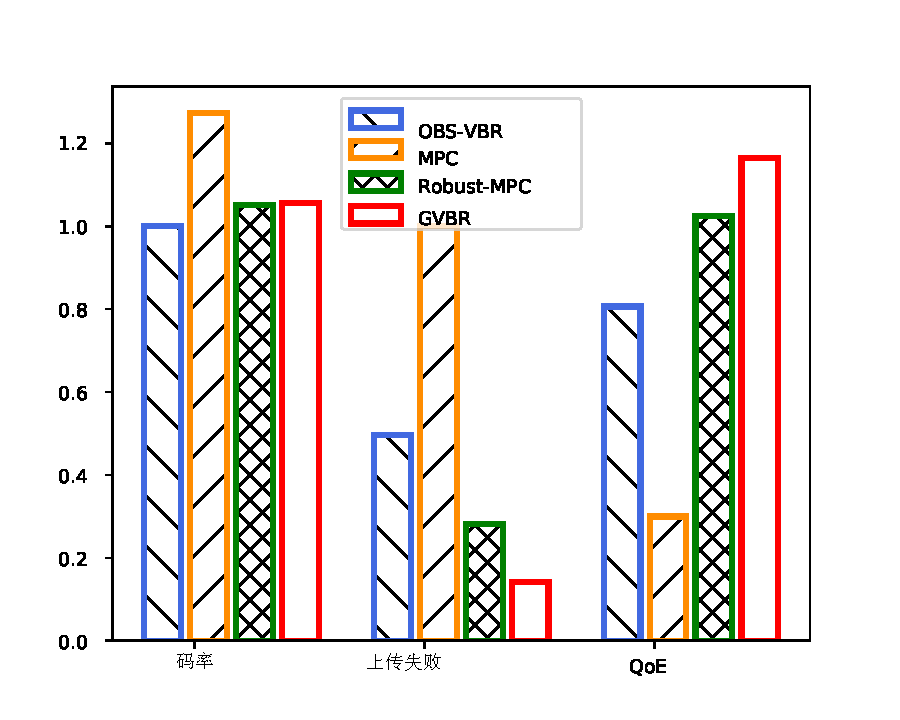
\includegraphics[width=\textwidth]{massive_qoe}
  \caption{归一化平均码率,上传失败时长和用户体验质量}
  \label{fig:massive_qoe}
\end{figure}

大规模的仿真结果展示在图~\ref{fig:massive_qoe}中,我们用两个数据集去评估GVBR算法,FCC数据集和HSDPA数据集。图中展示的用户体验质量是归一化的体验质量。在所有四种算法中,MPC有最大的码率用户体验,因为带宽估计算法很激进,MPC会更倾向于选择高码率。其他三种算法有些相同的平均码率,其中GVBR要稍微高一点。MPC有着最高的码率,也带来了最高的丢帧数,平均上传失败的时长最长。GVBR将平均上传失败的时长减少到很小,相对于Robust-MPC减少了50\%。有还不错的码率以及低的上传失败时长,GVBR明显是所有算法中最高的,达到了最高的用户体验质量。

\begin{figure}[htb]
  \centering%
  \begin{subfigure}{0.5\textwidth}
    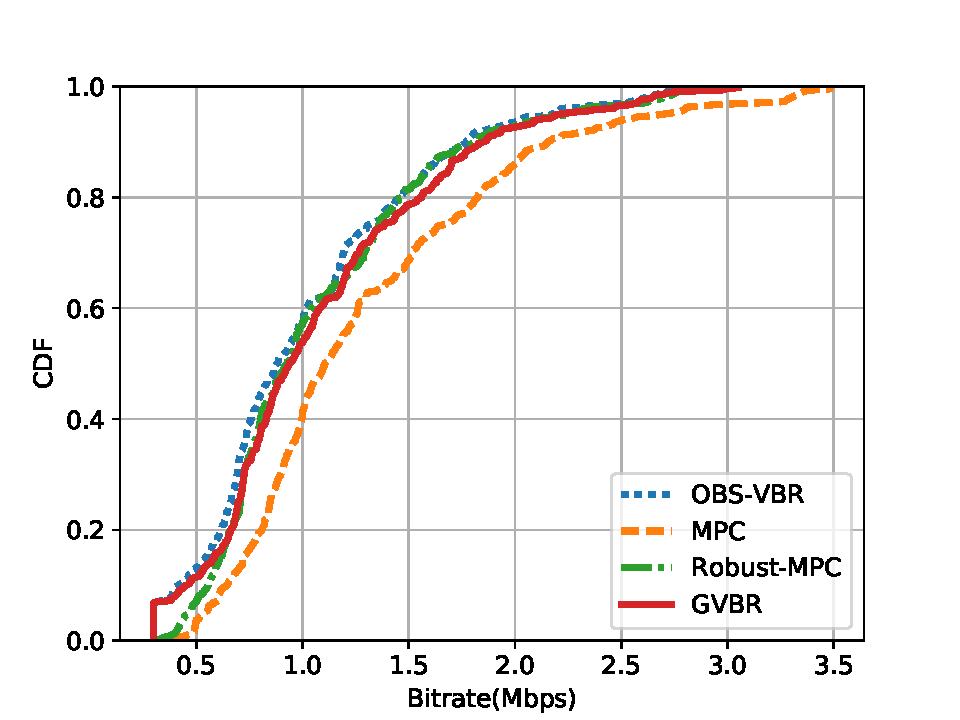
\includegraphics[width=\textwidth]{massive-bitrate-cdf}
    \caption{平均码率累计分布图}
    \label{fig:bitrate_cdf}
  \end{subfigure}%
  \vfill
  \vspace{0.2in}
  \begin{subfigure}{0.5\textwidth}
    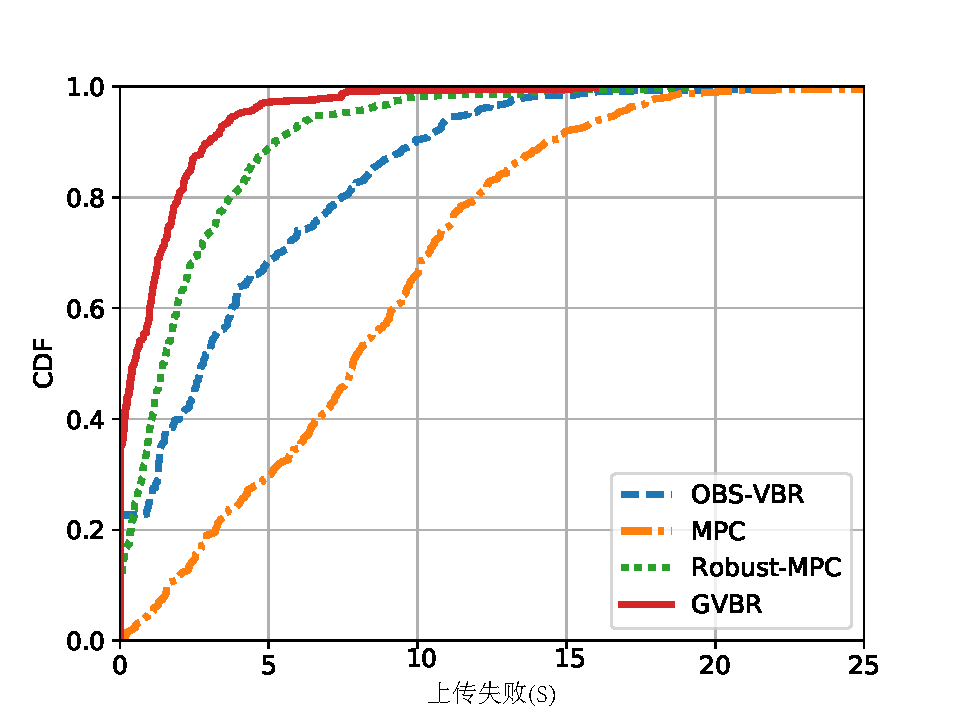
\includegraphics[width=\textwidth]{massive-drop-cdf}
    \caption{上传失败时长累计分布图}
    \label{fig:drop_cdf}
  \end{subfigure}
  \vfill
  \vspace{0.2in}
  \begin{subfigure}{0.5\textwidth}
    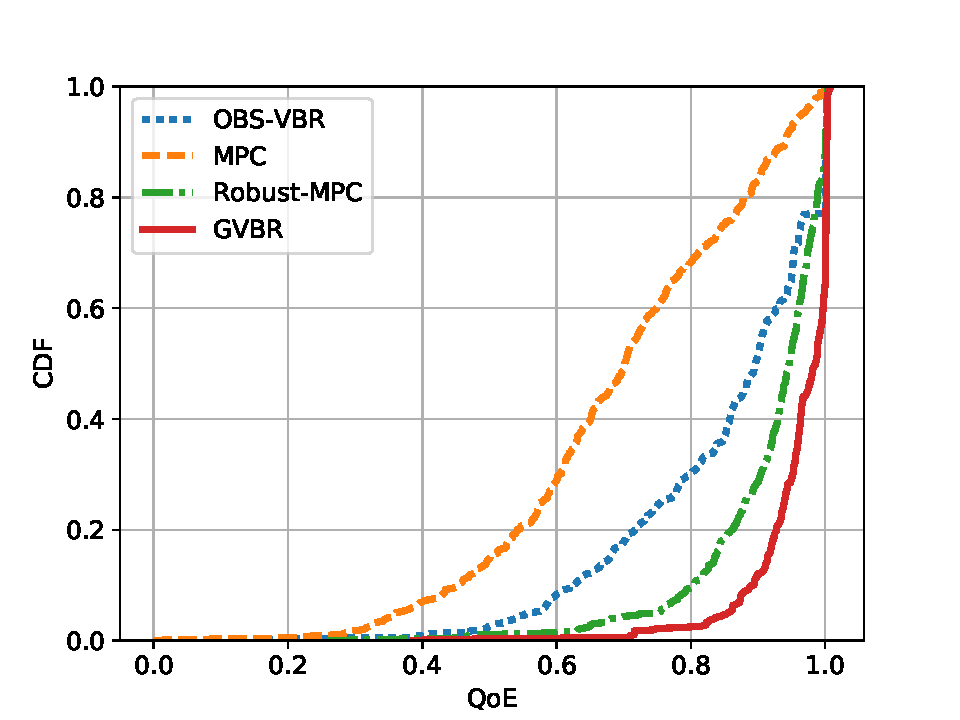
\includegraphics[width=\textwidth]{massive-qoe-cdf}
    \caption{归一化用户体验质量累计分布图}
    \label{fig:qoe_cdf}
  \end{subfigure}
  \caption{大规模实验结果图}
  \label{fig:massive_cdf}
\end{figure}

关于码率,上传失败时长和归一化用户体验质量的累计分布图展示在图~\ref{fig:massive_cdf}。在图~\ref{fig:bitrate_cdf}中,GVBR位于Robust-MPC和OBS的右边,码率稍微高于这两者。GVBR中,98\%的上传失败时间都低于5s,有大约40\%的的情况未出现上传失败。GVBR算法中,只有2\%的情况下用户体验质量不是很好,其余的98\%归一化用户体验质量大约在$[0.8,1]$之间。

相比于最原始的固定码率OBS算法,GVBR减少了96\%的丢帧。原始的OBS算法平均上传失败时长是26s,而我们的GVBR算法只有1s的平均失败时长。总的来说,我们的GVBR算法实现了更高的码率,在此同时显著减少了上传失败的发生。